\documentclass[10pt,letter,notitlepage]{article}
%Mise en page
\usepackage[left=2cm, right=2cm, lines=45, top=0.8in, bottom=0.7in]{geometry}
\usepackage{fancyhdr}
\usepackage{fancybox}
\usepackage{pdfpages} 
\renewcommand{\headrulewidth}{1.5pt}
\renewcommand{\footrulewidth}{1.5pt}
\pagestyle{fancy}
\newcommand\Loadedframemethod{TikZ}
\usepackage[framemethod=\Loadedframemethod]{mdframed}
\usepackage{tikz}
%\usepackage[linesnumbered,ruled,vlined]{algorithm2e}
%\usepackage{url}
\usepackage{dsfont}
\usepackage{amssymb,amsmath}
\usepackage{xspace}
\usepackage{comment}
\usepackage[shortlabels]{enumitem}



\usepackage{xcolor}


\usepackage{algorithm}
\usepackage[noend]{algpseudocode}

\lhead{
\textbf{Concordia University}
}
\rhead{\textbf{Fall 2024}
}
\chead{\textbf{
COMP6321
 }}

\newcommand{\RR}{\mathds{R}}
\newcommand{\sign}{\mathop{\mathrm{sign}}}
\newcommand{\argmin}{\mathop{\mathrm{argmin}}}
\newcommand{\zero}{\mathbf{0}}
\newcommand{\one}{\mathbf{1}}
\newcommand{\bv}{\mathbf{b}}
\newcommand{\wv}{\mathbf{w}}
\newcommand{\xv}{\mathbf{x}}
\newcommand{\yv}{\mathbf{y}}
\newcommand{\rv}{\mathbf{r}}
\newcommand{\inner}[2]{\langle #1, #2 \rangle}
\newcommand{\red}[1]{{\color{red}#1}}
\newcommand{\blue}[1]{{\color{blue}#1}}
\newcommand{\magenta}[1]{{\color{magenta}#1}}
\newcommand{\bits}{\{ 0, 1 \}}


\newcommand{\ea}{{et al.}\xspace}
\newcommand{\eg}{{e.g.}\xspace}
\newcommand{\ie}{{i.e.}\xspace}
\newcommand{\iid}{{i.i.d.}\xspace}
\newcommand{\cf}{{cf.}\xspace}
\newcommand{\wrt}{{w.r.t.}\xspace}
\newcommand{\aka}{{a.k.a.}\xspace}
\newcommand{\etc}{{etc.}\xspace}

\newcommand{\ans}[1]{{\color{orange}\textsf{Ans}: #1}}


\lfoot{}
\cfoot{\textbf{Parsa Kamalipour (\href{mailto:parsa.kamalipour@mail.concordia.ca}{parsa.kamalipour@mail.concordia.ca}) \textcopyright 2024}}

%================================
%================================

\setlength{\parskip}{1cm}
\setlength{\parindent}{1cm}
\tikzstyle{titregris} =
[draw=gray,fill=white, shading = exersicetitle, %
text=gray, rectangle, rounded corners, right,minimum height=.3cm]
\pgfdeclarehorizontalshading{exersicebackground}{100bp}
{color(0bp)=(green!40); color(100bp)=(black!5)}
\pgfdeclarehorizontalshading{exersicetitle}{100bp}
{color(0bp)=(red!40);color(100bp)=(black!5)}
\newcounter{exercise}
\renewcommand*\theexercise{exercice \textbf{Exercice}~n\arabic{exercise}}
\makeatletter
\def\mdf@@exercisepoints{}%new mdframed key:
\define@key{mdf}{exercisepoints}{%
\def\mdf@@exercisepoints{#1}
}

\mdfdefinestyle{exercisestyle}{%
outerlinewidth=1em,outerlinecolor=white,%
leftmargin=-1em,rightmargin=-1em,%
middlelinewidth=0.5pt,roundcorner=3pt,linecolor=black,
apptotikzsetting={\tikzset{mdfbackground/.append style ={%
shading = exersicebackground}}},
innertopmargin=0.1\baselineskip,
skipabove={\dimexpr0.1\baselineskip+0\topskip\relax},
skipbelow={-0.1em},
needspace=0.5\baselineskip,
frametitlefont=\sffamily\bfseries,
settings={\global\stepcounter{exercise}},
singleextra={%
\node[titregris,xshift=0.5cm] at (P-|O) %
{~\mdf@frametitlefont{\theexercise}~};
\ifdefempty{\mdf@@exercisepoints}%
{}%
{\node[titregris,left,xshift=-1cm] at (P)%
{~\mdf@frametitlefont{\mdf@@exercisepoints points}~};}%
},
firstextra={%
\node[titregris,xshift=1cm] at (P-|O) %
{~\mdf@frametitlefont{\theexercise}~};
\ifdefempty{\mdf@@exercisepoints}%
{}%
{\node[titregris,left,xshift=-1cm] at (P)%
{~\mdf@frametitlefont{\mdf@@exercisepoints points}~};}%
},
}
\makeatother


%%%%%%%%%

%%%%%%%%%%%%%%%
\mdfdefinestyle{theoremstyle}{%
outerlinewidth=0.01em,linecolor=black,middlelinewidth=0.5pt,%
frametitlerule=true,roundcorner=2pt,%
apptotikzsetting={\tikzset{mfframetitlebackground/.append style={%
shade,left color=white, right color=blue!20}}},
frametitlerulecolor=black,innertopmargin=1\baselineskip,%green!60,
innerbottommargin=0.5\baselineskip,
frametitlerulewidth=0.1pt,
innertopmargin=0.7\topskip,skipabove={\dimexpr0.2\baselineskip+0.1\topskip\relax},
frametitleaboveskip=1pt,
frametitlebelowskip=1pt
}
\setlength{\parskip}{0mm}
\setlength{\parindent}{10mm}
\mdtheorem[style=theoremstyle]{exercise}{\textbf{Exercise}}
\mdtheorem[style=theoremstyle]{Answer}{\textbf{Answers to Exercise}}
%================Liste definition--numList-and alphList=============
\newcounter{alphListCounter}
\newenvironment
{alphList}
{\begin{list}
{\alph{alphListCounter})}
{\usecounter{alphListCounter}
\setlength{\rightmargin}{0cm}
\setlength{\leftmargin}{0.5cm}
\setlength{\itemsep}{0.2cm}
\setlength{\partopsep}{0cm}
\setlength{\parsep}{0cm}}
}
{\end{list}}
\newcounter{numListCounter}
\newenvironment
{numList}
{\begin{list}
{\arabic{numListCounter})}
{\usecounter{numListCounter}
\setlength{\rightmargin}{0cm}
\setlength{\leftmargin}{0.5cm}
\setlength{\itemsep}{0cm}
\setlength{\partopsep}{0cm}
\setlength{\parsep}{0cm}}
}
{\end{list}}

\usepackage[breaklinks=true,letterpaper=true,linkcolor=magenta,urlcolor=magenta,citecolor=black]{hyperref}

\usepackage{cleveref}


%===========================================================
\begin{document}

\begin{center}
  \large{\textbf{COMP 6321 Machine Learning} \\ Assignment 4 Answers} \\


$Name:$ \href{https://benymaxparsa.github.io}{Parsa Kamalipour} \; , \; $Student ID:$ 40310734


\section{Exercise 1, Question 1: Introduction}
In this exercise, I had to implement the VGG11 convolutional neural network and train it on the MNIST dataset. The VGG11 model is a simpler version of the well-known VGG16 model. It has 11 layers with convolutional, batch normalization, and fully connected parts. The goal was to train the model to classify the digits from the MNIST dataset.

\section{Exercise 1, Question 1: Methodology}

\subsection{Environment Setup}
I implemented the model in Python using PyTorch. I made sure that the code works for different hardware setups:
\begin{itemize}
    \item CUDA (for systems with an NVIDIA GPU)
    \item MPS (for Apple Silicon devices like M1, M2)
    \item CPU (if no GPU is available)
\end{itemize}

The following dependencies were used:
\begin{itemize}
    \item \texttt{torch}
    \item \texttt{torchvision}
    \item \texttt{numpy}
\end{itemize}

\subsection{MNIST Dataset}
The MNIST dataset was loaded using the \texttt{torchvision.datasets} module. The images were resized from $28 \times 28$ to $32 \times 32$ to match the VGG input size. The dataset was split into training and testing sets, and normalization was applied.

\subsection{Model Architecture}
The VGG11 model that I implemented for this experiment consists of these layers:
\begin{itemize}
    \item Convolutional layers with batch normalization and ReLU activation
    \item Max pooling layers after some convolutional layers
    \item Fully connected layers with ReLU activation and Dropout
    \item Output layer with 10 units for the classes (digits 0-9)
\end{itemize}

The model uses the following configuration for the convolutional and fully connected layers:
\begin{verbatim}
- Conv(1, 64, 3, 1, 1) - BatchNorm(64) - ReLU - MaxPool(2, 2)
- Conv(64, 128, 3, 1, 1) - BatchNorm(128) - ReLU - MaxPool(2, 2)
- Conv(128, 256, 3, 1, 1) - BatchNorm(256) - ReLU
- Conv(256, 256, 3, 1, 1) - BatchNorm(256) - ReLU - MaxPool(2, 2)
- Conv(256, 512, 3, 1, 1) - BatchNorm(512) - ReLU
- Conv(512, 512, 3, 1, 1) - BatchNorm(512) - ReLU - MaxPool(2, 2)
- Conv(512, 512, 3, 1, 1) - BatchNorm(512) - ReLU
- Conv(512, 512, 3, 1, 1) - BatchNorm(512) - ReLU - MaxPool(2, 2)
- Linear(512, 4096) - ReLU - Dropout(0.5)
- Linear(4096, 4096) - ReLU - Dropout(0.5)
- Linear(4096, 10)
\end{verbatim}

\section{Exercise 1, Question 1: Training Process}
The model was trained with the following settings:
\begin{itemize}
    \item Loss function: Cross-entropy loss (\texttt{torch.nn.CrossEntropyLoss})
    \item Optimizer: Stochastic Gradient Descent (SGD) with learning rate $0.01$ and momentum $0.9$
    \item Number of epochs: 20
    \item Batch size: 64
\end{itemize}

The model was trained for 20 epochs, and I printed the training loss periodically to track the progress. The training loop involved zeroing gradients, forward propagation, computing the loss, backward propagation, and updating the parameters.

\section{Exercise 1, Question 1: Results}
The model was successfully trained for 20 epochs. The training process showed that the loss decreased steadily, which means the model was learning to classify the digits correctly. I saved the trained model for future evaluation and testing.

\section{Exercise 1, Question 2: Introduction}
In this exercise, I needed to evaluate the training process of the VGG11 model, which I implemented in Question 1, on the MNIST dataset. The goal was to analyze the model's performance by plotting both the training and testing accuracies, as well as the training and testing losses for each epoch. This helps me understand how well the model is learning and how it generalizes.

\section{Exercise 1, Question 2: Methodology}
I used Python and PyTorch to perform the evaluation. The model that I trained earlier was loaded, and I evaluated it using both the training and test datasets. For the evaluation, I stored the training loss, test loss, training accuracy, and test accuracy for each epoch.

\subsection{Environment Setup}
I ran the evaluation using the same environment setup as before, where the hardware setup included:
\begin{itemize}
    \item CUDA (for systems with NVIDIA GPU)
    \item MPS (for Apple Silicon devices like M1, M2)
    \item CPU (if no GPU is available)
\end{itemize}

\subsection{Evaluation Procedure}
The model was evaluated for 20 epochs. In each epoch, I:
\begin{itemize}
    \item Trained the model and computed the training loss.
    \item Evaluated the training accuracy by checking how well the model predicted labels on the training data.
    \item Evaluated the test accuracy and test loss by using the model on the test data without updating the weights.
\end{itemize}

The metrics were calculated using the following functions:
\begin{itemize}
    \item \texttt{calculate\_accuracy}: This function calculates the percentage of correct predictions out of the total samples.
    \item \texttt{calculate\_loss}: This function computes the average loss across all samples.
\end{itemize}

\section{Exercise 1, Question 2: Results}
The evaluation process showed how the model's accuracy and loss evolved over time.
\begin{itemize}
    \item The training accuracy and test accuracy were recorded at the end of each epoch.
    \item The training and test loss were also recorded to see if the model was converging well.
\end{itemize}

The graphs for the training and test accuracy and loss are shown in Figures \ref{fig:accuracy} and \ref{fig:loss}.

\begin{figure}[H]
    \centering
    \begin{minipage}{0.45\textwidth}
        \centering
        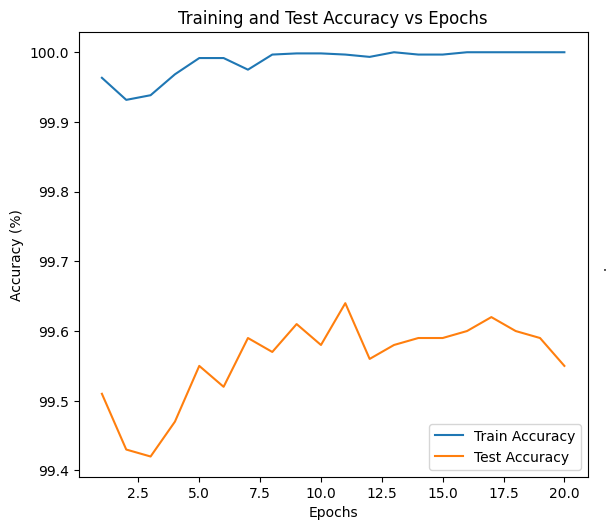
\includegraphics[width=\textwidth]{training_test_accuracy.png}
        \caption{Training and Test Accuracy vs Epochs}
        \label{fig:accuracy}
    \end{minipage}
    \hfill
    \begin{minipage}{0.45\textwidth}
        \centering
        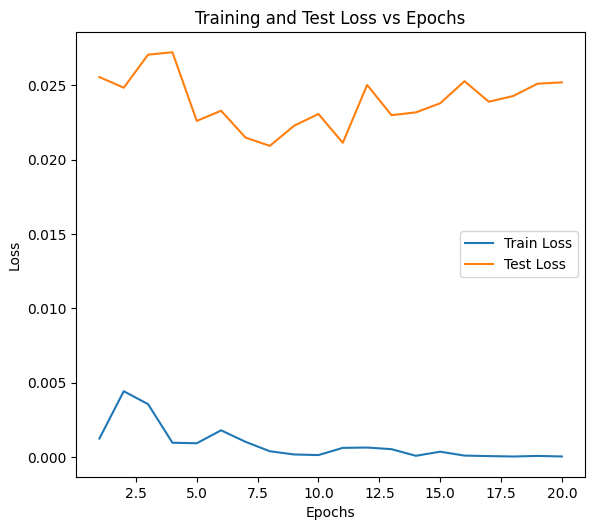
\includegraphics[width=\textwidth]{training_test_loss.png}
        \caption{Training and Test Loss vs Epochs}
        \label{fig:loss}
    \end{minipage}
    \caption{Training and Test Metrics for VGG11 Model on MNIST}
    \label{fig:results}
\end{figure}

The results show that the training accuracy was very high, almost reaching 100\% throughout the epochs, while the test accuracy was slightly lower and fluctuated between 99.4\% and 99.7\%. This indicates that the model performed well on the training data but had some difficulty generalizing to new data.

The training loss was very low and approached zero by the end of the training, which means the model was fitting the training data very well. However, the test loss was higher and fluctuated, suggesting that the model had some challenges generalizing perfectly to the test data. The fluctuations in test accuracy and loss indicate that while the model was effective, there was still some room for improvement in terms of generalization.

The graphs also helped me check if the model was overfitting. Although the training accuracy was higher than the test accuracy, the difference was not too large, suggesting that overfitting was not severe, but there was some overfitting present.

\section{Exercise 1, Question 2: Conclusion}
From the evaluation, I observed that the VGG11 model was able to learn the MNIST dataset quite well over the course of 20 epochs. The training accuracy was consistently high, and the training loss decreased significantly. However, the test accuracy was lower than the training accuracy, and the test loss fluctuated, indicating that the model's ability to generalize was not perfect, and some overfitting might be present.

\section{Exercise 1, Question 3: Introduction}
In this part of the exercise, I evaluated the generalization capabilities of the VGG11 model on the MNIST dataset under different transformations. The goal was to understand how well the model performs when test images are flipped, blurred, or have Gaussian noise added to them. By doing this, I wanted to see how robust the model is to changes in the input data that it did not encounter during training.

\section{Exercise 1, Question 3: Methodology}
The model was evaluated on the original MNIST test set as well as on versions of the test set that were transformed in several ways:
\begin{itemize}
    \item \textbf{Horizontal Flip}: Images were flipped from left to right.
    \item \textbf{Vertical Flip}: Images were flipped from top to bottom.
    \item \textbf{Combined Horizontal and Vertical Flip}: Images were flipped both horizontally and vertically.
    \item \textbf{Gaussian Blur}: Images were blurred with a Gaussian filter.
    \item \textbf{Gaussian Noise}: Gaussian noise was added to the images with variances of 0.01, 0.1, and 1.
\end{itemize}
The VGG11 model was evaluated on each of these transformed datasets, and the test accuracy was calculated for each transformation.

\section{Exercise 1, Question 3: Results}
The results of the evaluation are summarized in Table \ref{tab:results}.

\begin{table}[H]
    \centering
    \begin{tabular}{|l|c|}
        \hline
        \textbf{Transformation} & \textbf{Accuracy (\%)} \\
        \hline
        Original Test Set & 99.09 \\
        Horizontally Flipped Test Set & 38.49 \\
        Vertically Flipped Test Set & 41.79 \\
        Horizontally and Vertically Flipped Test Set & 42.06 \\
        Blurred Test Set & 97.65 \\
        Gaussian Noise (Variance 0.01) & 99.09 \\
        Gaussian Noise (Variance 0.1) & 98.84 \\
        Gaussian Noise (Variance 1) & 10.55 \\
        \hline
    \end{tabular}
    \caption{Test accuracy of VGG11 on different transformations of the MNIST dataset.}
    \label{tab:results}
\end{table}

\begin{figure}[H]
  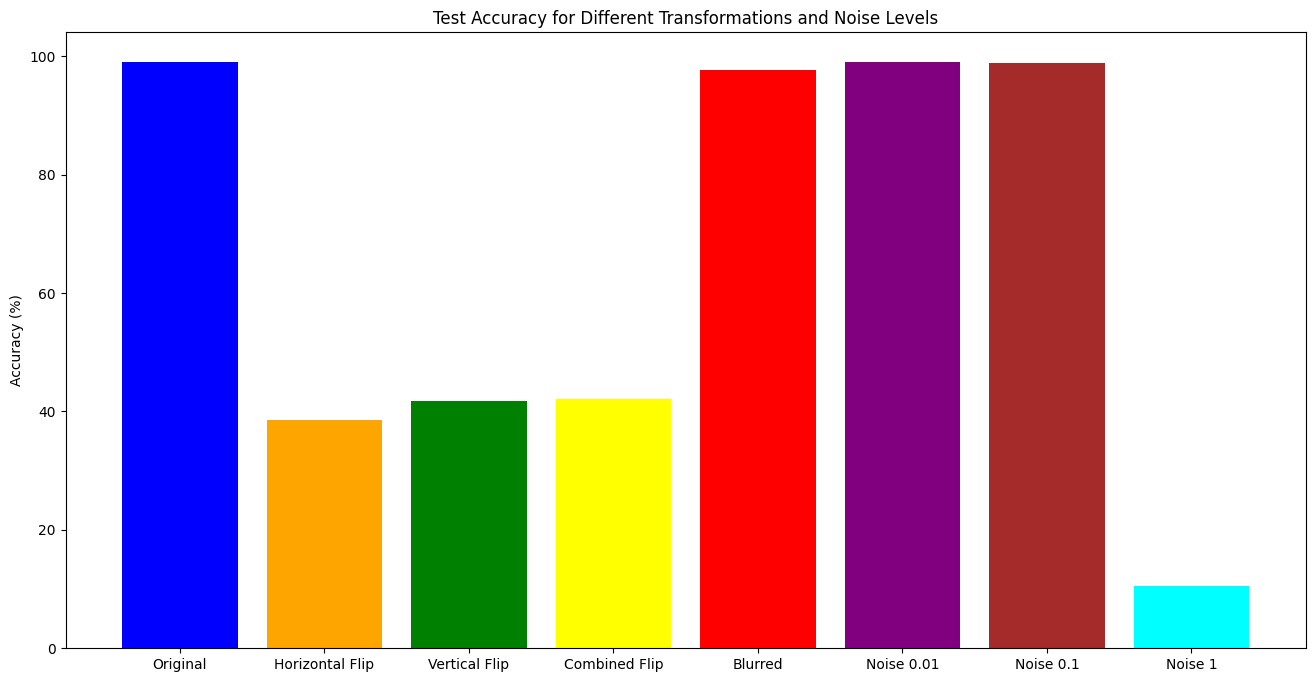
\includegraphics[width=\textwidth]{diffTransformNoise.png}
  \caption{Plot accuracies for better visualization}
\end{figure}


\section{Exercise 1, Question 3: Analysis}
The results show that the VGG11 model performed very well on the original MNIST test set, achieving an accuracy of 99.09\%. The model also handled small levels of Gaussian noise (variance 0.01 and 0.1) quite well, with accuracies of 99.09\% and 98.84\%, respectively. However, when the noise level was increased to a variance of 1, the model's accuracy dropped drastically to 10.55\%. This suggests that the model struggles with high levels of noise.

The model's performance on horizontally and vertically flipped images was significantly lower, with accuracies of 38.49\%, 41.79\%, and 42.06\% for horizontal, vertical, and combined flips, respectively. This indicates that the model is not invariant to image flips, likely because it was not trained on flipped versions of the images. The accuracy on blurred images was 97.65\%, showing that the model is relatively robust to minor blurring.

\section{Exercise 1, Question 3: Conclusion}
The evaluation shows that the VGG11 model is highly accurate on the original MNIST test set and is also fairly robust to small levels of Gaussian noise and blurring. However, the model struggles with flipped images and high levels of noise. This suggests that the model's training did not include sufficient variations of the data to handle these transformations effectively.

\section{Exercise 1, Question 4: Introduction}
In this part of the exercise, I retrained the VGG11 model on the MNIST dataset, but this time I applied different data augmentation techniques. The goal was to observe how data augmentation helps the model generalize better and how it affects the overall performance. I used transformations such as random horizontal flips, rotations, affine transformations, and color jitter to make the training data more diverse and challenging.

\section{Exercise 1, Question 4: Methodology}
For the retraining, I used the following data augmentation techniques:
\begin{itemize}
    \item \textbf{Random Horizontal Flip}: Randomly flipped images horizontally with a 50\% probability.
    \item \textbf{Random Rotation}: Applied random rotations up to 10 degrees.
    \item \textbf{Random Affine Transformation}: Applied affine transformations with translations of up to 10\% of the image.
    \item \textbf{Color Jitter}: Adjusted brightness, contrast, saturation, and hue with small variations to make the images appear different.
\end{itemize}

The training was done for 20 epochs, and the loss was calculated at each mini-batch. I also evaluated the model on the test set after each epoch to observe the changes in accuracy.

\section{Exercise 1, Question 4: Results}
The final test accuracy after retraining the model with data augmentation was 99.03\%, which is slightly lower compared to the original training without data augmentation. The training loss fluctuated throughout the epochs, indicating that the model faced challenges in some mini-batches, but overall it was able to learn effectively. Below are the training and test metrics observed during the retraining process.

\begin{figure}[H]
    \centering
    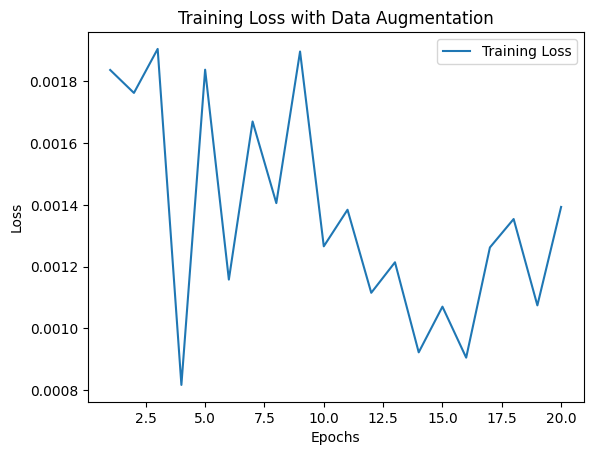
\includegraphics[width=0.8\textwidth]{TrainingAug.png}
    \caption{Training Loss over 20 Epochs with Data Augmentation}
    \label{fig:train_loss_plot}
\end{figure}

Figure \ref{fig:train_loss_plot} shows the fluctuation in training loss over the epochs. The model managed to achieve a good level of learning despite the variations in the loss. The test accuracy was consistently high, around 99\%, throughout the retraining process, which shows that the data augmentation did not hurt the model's performance.

\section{Exercise 1, Question 4: Analysis}
The results show that the VGG11 model, even with augmented data, maintained a high level of accuracy on the MNIST test set. Although the final test accuracy was slightly lower compared to the training without augmentation, I believe this slight drop is because the augmented data makes learning more challenging, which prevents overfitting. The diverse augmented images allowed the model to learn more general features, which is beneficial for better generalization.

\section{Exercise 1, Question 4: Conclusion}
Retraining the VGG11 model with data augmentation showed that the model could still achieve a high accuracy of 99.03\% on the test set. The training loss fluctuated, and the test accuracy remained high, which suggests that data augmentation helped the model learn more robust features and avoid overfitting. This confirms that data augmentation is an effective way to improve the generalization capabilities of deep learning models.


\section{Exercise 1, Question 5: Introduction}
In this part of Exercise 1, I compared the performance of three different optimizers (AdaDelta, Adam, and SGD) while training the VGG11 model on the MNIST dataset. The objective was to see how each optimizer affected the accuracy and convergence during training and on the test set.

\section{Exercise 1, Question 5: Methodology}
For training, I used the following three optimizers:
\begin{itemize}
    \item \textbf{AdaDelta}: Used with a learning rate of 1.0.
    \item \textbf{Adam}: Used with a learning rate of 0.001.
    \item \textbf{SGD (Stochastic Gradient Descent)}: Used with a learning rate of 0.01 and momentum of 0.9.
\end{itemize}

I trained each model for 20 epochs, tracking both the training and test accuracies after each epoch. The results were plotted to compare the performances visually.

\section{Exercise 1, Question 5: Results}
The training accuracy and test accuracy results for all three optimizers over 20 epochs are shown in the figures below.

\begin{figure}[H]
    \centering
    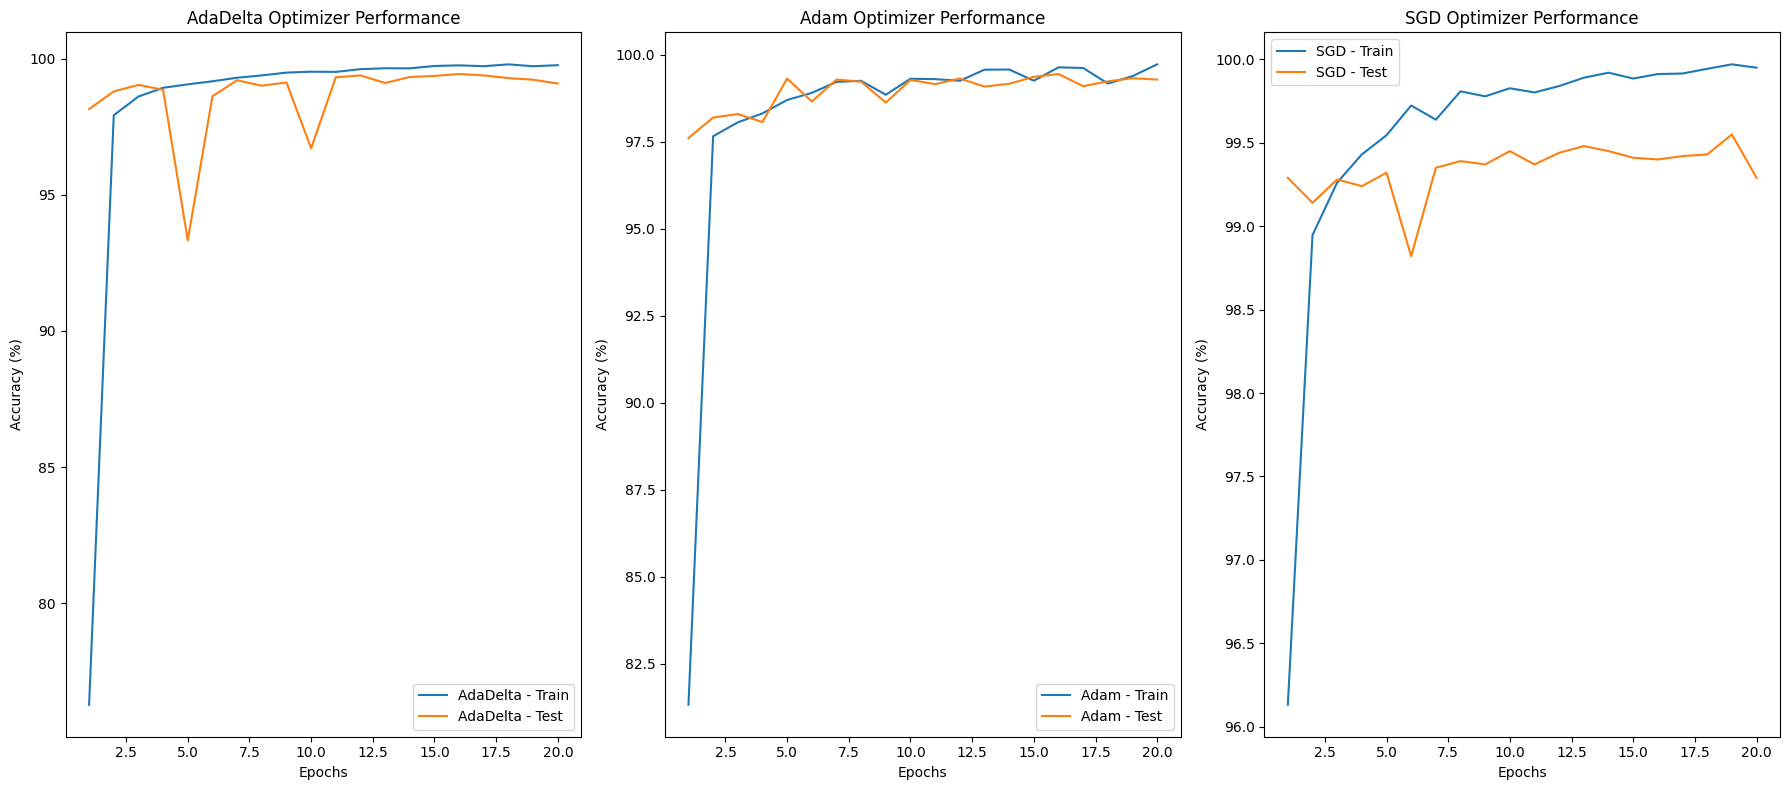
\includegraphics[width=1\textwidth]{1.5.1.png}
    \caption{Training and Test Accuracies for AdaDelta, Adam, and SGD Optimizers}
    \label{fig:optimizer_performance}
\end{figure}

The performance of each optimizer was also compared in a combined plot, which is shown in Figure \ref{fig:optimizer_comparison}.

\begin{figure}[H]
    \centering
    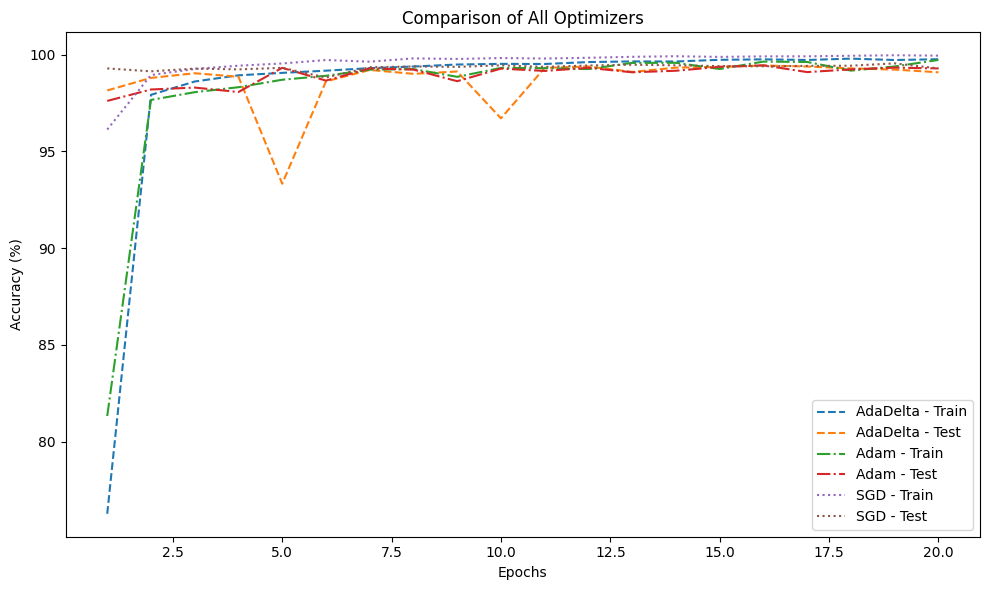
\includegraphics[width=0.8\textwidth]{1.5.2.png}
    \caption{Comparison of All Optimizers (AdaDelta, Adam, SGD)}
    \label{fig:optimizer_comparison}
\end{figure}

\section{Exercise 1, Question 5: Analysis}
Based on the training results, the final test accuracy for each optimizer was as follows:
\begin{itemize}
    \item \textbf{AdaDelta}: Achieved a maximum test accuracy of 99.44\%. Test accuracy fluctuated during training, with a notable dip in epoch 5 (93.33\%).
    \item \textbf{Adam}: Achieved a maximum test accuracy of 99.45\%. The accuracy was mostly consistent, with a slight dip in epoch 9 (98.63\%).
    \item \textbf{SGD}: Achieved a maximum test accuracy of 99.55\%. It showed a steady improvement and had the highest overall accuracy.
\end{itemize}

The SGD optimizer showed the highest final test accuracy, while both AdaDelta and Adam also performed quite well. SGD seemed to converge to a high accuracy more steadily compared to AdaDelta, which had fluctuations in the test accuracy during training. Adam also showed a stable performance similar to SGD, but with a slightly slower convergence.

From the results:
\begin{itemize}
    \item 	\textbf{AdaDelta} started with a lower training accuracy (76.27\%) but quickly improved, reaching a high training accuracy of 99.77\%. However, it had some instability in the test accuracy during training.
    \item 	\textbf{Adam} had a more stable training process, starting with a training accuracy of 81.33\% and achieving 99.73\% by the end of training. The test accuracy remained mostly consistent.
    \item 	\textbf{SGD} started with a high training accuracy (96.13\%) and reached 99.95\% by the end of training. It achieved the best final test accuracy (99.55\%) and showed consistent improvement throughout the training process.
\end{itemize}

In my opinion, the SGD optimizer is better for this dataset because it reached the highest accuracy and had a more consistent performance across the epochs. However, both Adam and AdaDelta are good choices as they also achieved high accuracy, and they might be preferred in other scenarios due to their adaptive learning rate capabilities.

\section{Exercise 1, Question 6: Introduction}
In this part of Exercise 1, I replaced the ReLU activations in the VGG11 model with Sigmoid activations. The objective was to understand the impact of using Sigmoid activations compared to ReLU on the training and test accuracies of the model.

\section{Exercise 1, Question 6: Methodology}
I trained the VGG11 model using Sigmoid activation functions in place of ReLU. The optimizer used for training was Stochastic Gradient Descent (SGD) with a learning rate of 0.01 and momentum of 0.9, similar to what was used in Exercise 1.2. The model was trained for 20 epochs, and the results for both training and test accuracies were plotted for analysis.

\section{Exercise 1, Question 6: Results}
The training and test accuracies of the model with Sigmoid activations are shown in Figure \ref{fig:sigmoid_performance}.

\begin{figure}[H]
    \centering
    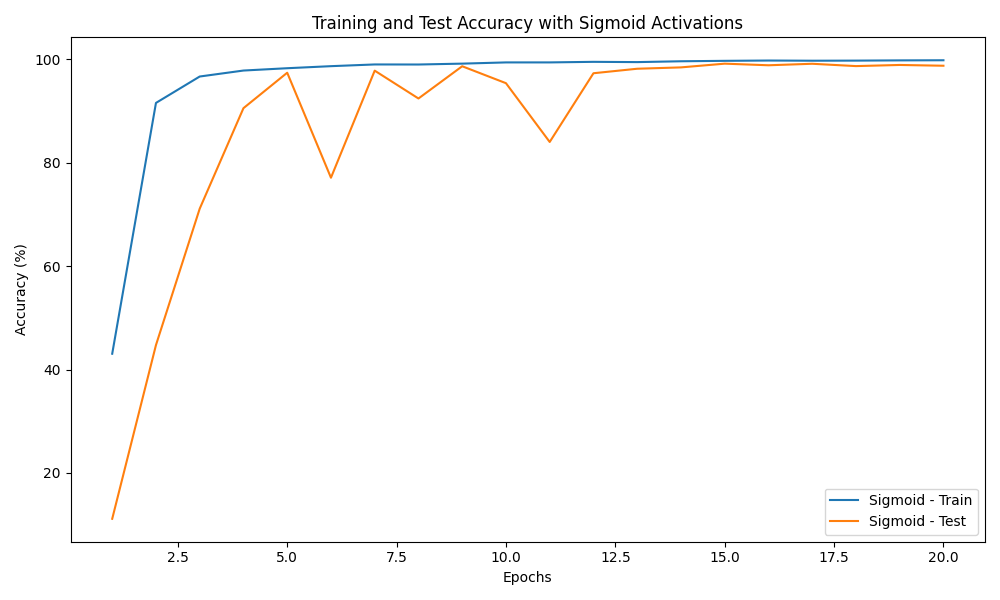
\includegraphics[width=0.8\textwidth]{sigmoid_activation_performance.png}
    \caption{Training and Test Accuracy with Sigmoid Activations}
    \label{fig:sigmoid_performance}
\end{figure}

The comparison between the Sigmoid and ReLU activation functions is shown in Figure \ref{fig:relu_vs_sigmoid}.

\begin{figure}[H]
    \centering
    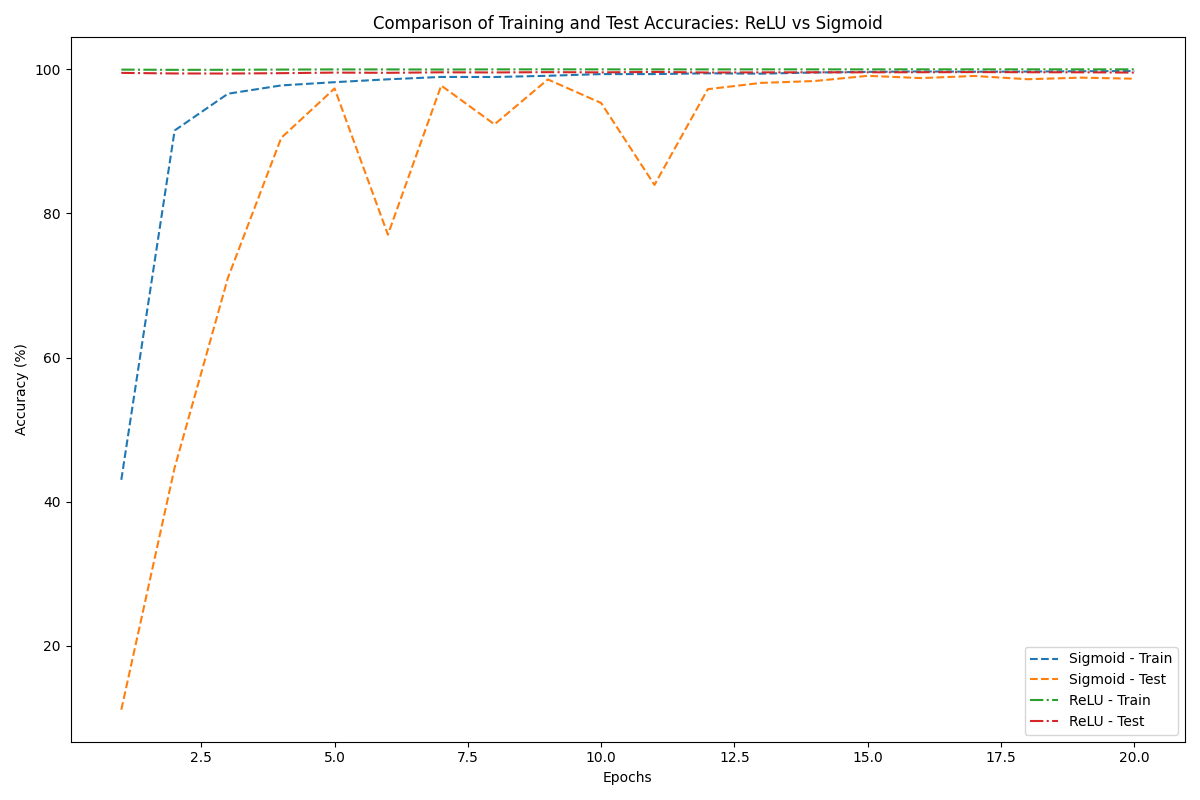
\includegraphics[width=0.8\textwidth]{comparison_relu_sigmoid.png}
    \caption{Comparison of Training and Test Accuracies: ReLU vs Sigmoid}
    \label{fig:relu_vs_sigmoid}
\end{figure}

\section{Exercise 1, Question 6: Analysis}
Based on the training results, I observed significant differences between the performance of Sigmoid and ReLU activations:
\begin{itemize}
    \item \textbf{Training Accuracy}: The Sigmoid model eventually reached a high training accuracy (99.76\%), similar to the ReLU model. However, it started with a lower initial accuracy and took more epochs to converge compared to the ReLU model.
    \item \textbf{Test Accuracy}: The test accuracy for the Sigmoid model fluctuated more compared to the ReLU model. The Sigmoid activation caused the model to struggle with generalization, especially in the earlier epochs, as evident by the dips in accuracy (e.g., in Epochs 6, 11).
    \item \textbf{Comparison}: ReLU activations performed better overall, with more stable and higher test accuracy. The Sigmoid model had issues like vanishing gradients, which made convergence slower and less consistent.
\end{itemize}

The ReLU model maintained a more consistent and higher test accuracy throughout training. Sigmoid activations tend to suffer from the vanishing gradient problem, which affects the learning capability of deep networks like VGG11. This explains the slower convergence and fluctuating test accuracy observed in the Sigmoid model.

\section{Exercise 1, Question 6: Conclusion}
In conclusion, the comparison showed that ReLU is a more suitable activation function for the VGG11 model on the MNIST dataset. ReLU provided better convergence and higher stability in both training and testing phases, whereas Sigmoid activations led to slower convergence and fluctuating test accuracy due to the vanishing gradient issue.

\section{Exercise 1, Question 7: Introduction}
In this part of Exercise 1, I removed the Dropout layers from the VGG11 model and trained the model again. The goal was to compare the performance of the model without Dropout with the model from Exercise 1.2, which had Dropout layers. This helped me understand how the presence or absence of Dropout affects the network's ability to generalize.

\section{Exercise 1, Question 7: Methodology}
I trained the VGG11 model without any Dropout layers. The optimizer used was Stochastic Gradient Descent (SGD) with a learning rate of 0.01 and a momentum of 0.9, the same as in Exercise 1.2. The model was trained for 20 epochs, and the results for both training and test accuracies were plotted for analysis.

\section{Exercise 1, Question 7: Results}
The training and test accuracies of the model without Dropout are shown in Figure \ref{fig:nodropout_performance}.

\begin{figure}[H]
    \centering
    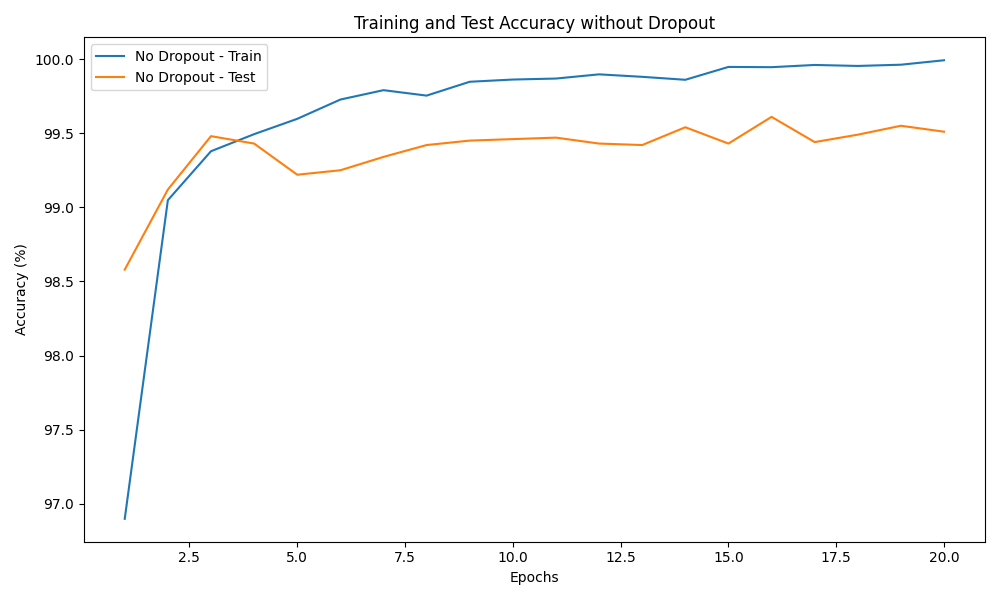
\includegraphics[width=0.8\textwidth]{nodropout_performance.png}
    \caption{Training and Test Accuracy without Dropout}
    \label{fig:nodropout_performance}
\end{figure}

The comparison between the model without Dropout and the model with Dropout from Exercise 1.2 is shown in Figure \ref{fig:relu_vs_nodropout}.

\begin{figure}[H]
    \centering
    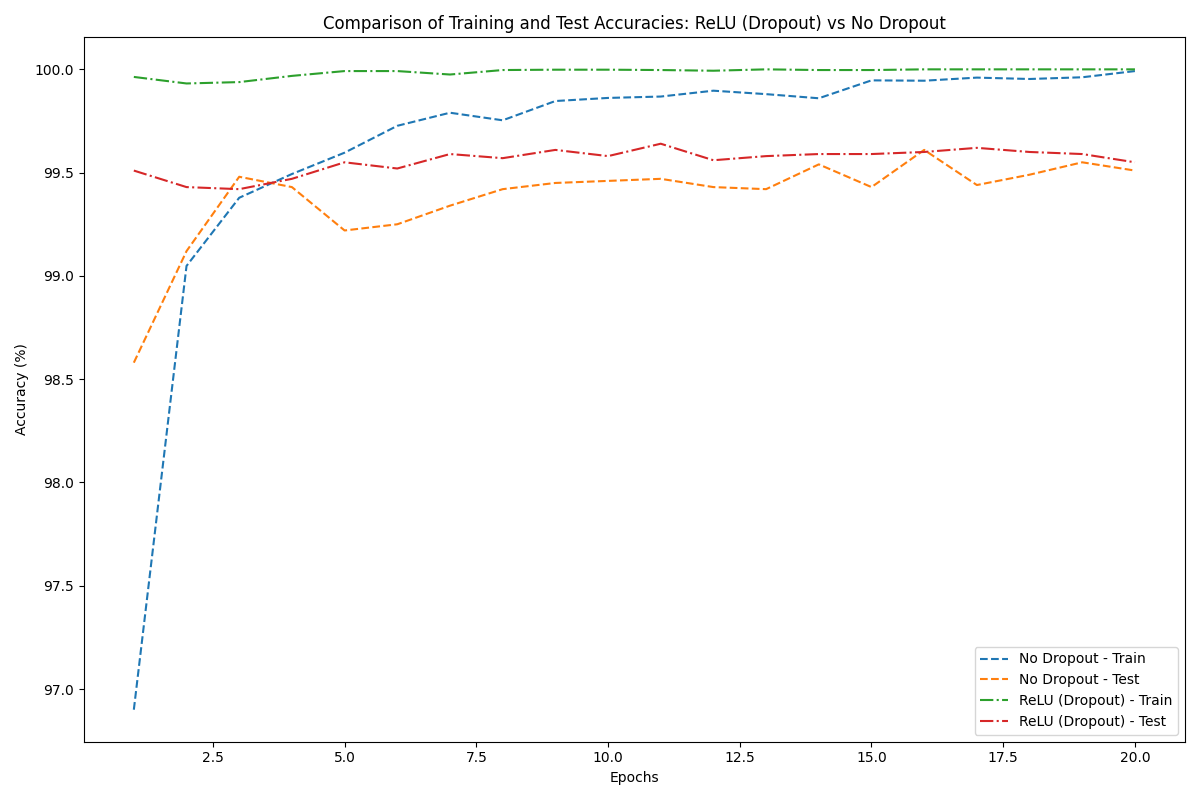
\includegraphics[width=0.8\textwidth]{comparison_relu_nodropout.png}
    \caption{Comparison of Training and Test Accuracies: ReLU (Dropout) vs No Dropout}
    \label{fig:relu_vs_nodropout}
\end{figure}

\section{Exercise 1, Question 7: Analysis}
Based on the training results, I observed significant differences between the performance of the model with and without Dropout:
\begin{itemize}
    \item \textbf{Training Accuracy}: The model without Dropout reached almost perfect training accuracy (99.99\%) by the end of the 20 epochs. This indicates that the model was able to memorize the training data very well without the regularization effects of Dropout.
    \item \textbf{Test Accuracy}: The test accuracy without Dropout was also quite high, reaching a peak of 99.61\%. However, it showed some minor fluctuations across epochs, suggesting that the model may have overfitted to the training data, which is something Dropout typically helps prevent.
    \item \textbf{Comparison}: The model with Dropout had a more consistent performance in both training and testing. Dropout helps in preventing the model from becoming too reliant on specific features, which often leads to better generalization. The model without Dropout had a higher training accuracy but was slightly less stable in terms of test accuracy, indicating a tendency towards overfitting.
\end{itemize}

The presence of Dropout layers made the model more robust and helped it generalize better to unseen data, while the model without Dropout tended to memorize the training data, leading to slightly less consistent test accuracy.

\section{Exercise 2, Question 1: Introduction}
In this part of Exercise 2, I implemented a three-layer Multi-Layer Perceptron (MLP) using PyTorch and trained it on the MNIST dataset. The architecture consisted of three fully connected layers with ReLU activations, Batch Normalization, and an output layer for classification.

\section{Exercise 2, Question 1: Methodology}
The MLP model was trained with the following structure:
\begin{itemize}
    \item \textbf{Layer 1}: A fully connected layer from 784 (flattened 28x28 images) to 512 units, followed by a ReLU activation function.
    \item \textbf{Layer 2}: A fully connected layer from 512 to 512 units, followed by Batch Normalization and a ReLU activation function.
    \item \textbf{Layer 3}: A fully connected layer from 512 to 10 units, corresponding to the 10 possible digit classes.
\end{itemize}

The loss function used was Cross-Entropy Loss, and the optimizer was Stochastic Gradient Descent (SGD) with a learning rate of 0.01 and a momentum of 0.9. The model was trained for 20 epochs, and both training and test accuracies were recorded for analysis.

\section{Exercise 2, Question 1: Results}
The training and test accuracies of the MLP model are shown in Figure \ref{fig:mlp_performance}.

\begin{figure}[h]
    \centering
    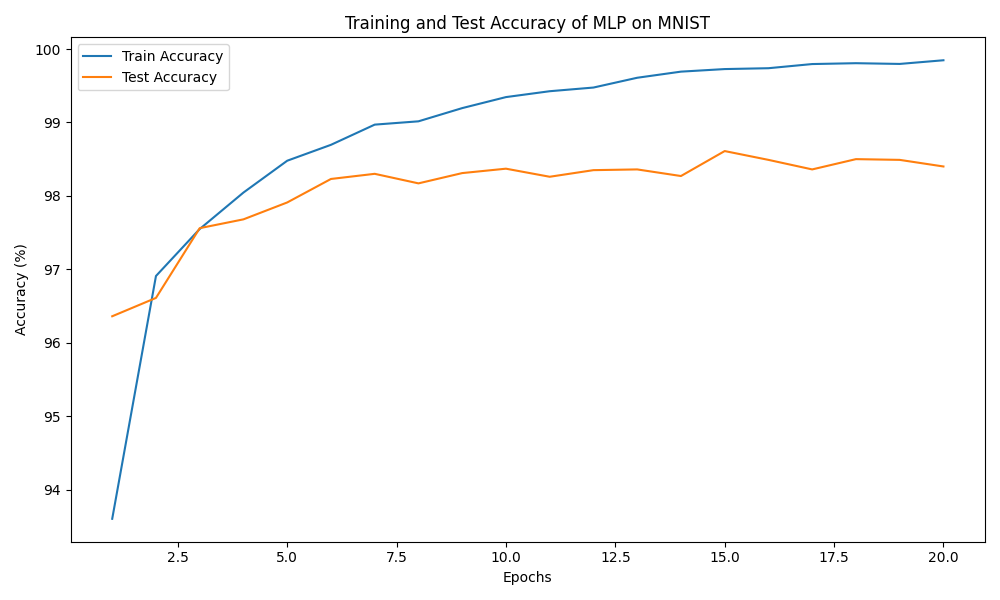
\includegraphics[width=0.8\textwidth]{mlp_performance.png}
    \caption{Training and Test Accuracy of MLP on MNIST}
    \label{fig:mlp_performance}
\end{figure}

\section{Exercise 2, Question 1: Analysis}
Based on the training results, I observed the following:
\begin{itemize}
    \item \textbf{Training Accuracy}: The training accuracy increased steadily over the 20 epochs, reaching almost perfect accuracy (99.94\%) by the end. This shows that the model was able to learn the training data well.
    \item \textbf{Test Accuracy}: The test accuracy also improved, reaching a maximum of 98.48\%. However, there was a noticeable gap between the training and test accuracies, especially in the later epochs. This indicates that the model might be slightly overfitting to the training data.
    \item \textbf{Overfitting}: The test accuracy plateaued around 98.4\% with slight fluctuations in the later epochs, which is a sign of overfitting. The model seems to be memorizing the training data rather than generalizing well to unseen data.
    \item \textbf{MLP Limitations}: Compared to deeper models like Convolutional Neural Networks (CNNs), the MLP with only fully connected layers may not capture spatial features of images as effectively. This could be one reason why the test accuracy did not reach the levels observed in more complex models like VGG11.
\end{itemize}

\section{Exercise 2, Question 2: Introduction}
In this part of Exercise 2, I trained the Multi-Layer Perceptron (MLP) on the MNIST dataset for 20 epochs and then created four plots to visualize the training process. The plots included: (a) Test accuracy vs. epochs, (b) Training accuracy vs. epochs, (c) Test loss vs. epochs, and (d) Training loss vs. epochs. These plots helped me understand the model's behavior during training and testing.

\section{Exercise 2, Question 2: Results and Analysis}
The results of the training process are shown in Figure \ref{fig:mlp_training_plots}. Based on these plots, I made several observations:

\begin{figure}[h]
    \centering
    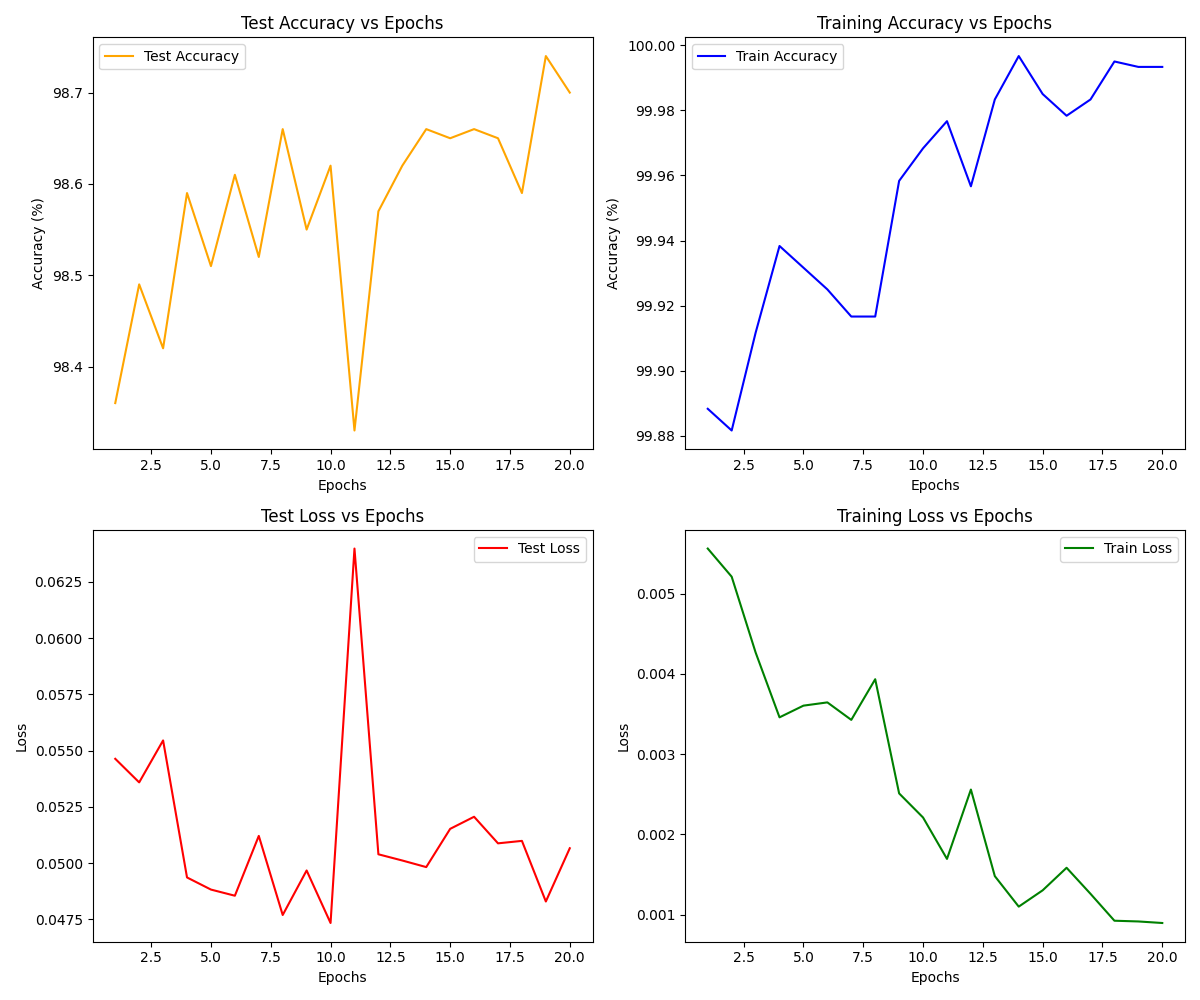
\includegraphics[width=0.8\textwidth]{mlp_training_plots.png}
    \caption{Training and Test Accuracy and Loss Plots for MLP on MNIST}
    \label{fig:mlp_training_plots}
\end{figure}

\subsection{Test Accuracy vs. Epochs}
The test accuracy fluctuated during training, ranging between approximately 98.35\% and 98.65\%. This fluctuation suggests that the model had some difficulty generalizing consistently on the test set, which might indicate some overfitting to the training data.

\subsection{Training Accuracy vs. Epochs}
The training accuracy steadily increased over the epochs, approaching 100\% by the end of training. This indicates that the model was able to learn the training data very well. However, the nearly perfect training accuracy compared to the fluctuating test accuracy is a potential sign of overfitting.

\subsection{Test Loss vs. Epochs}
The test loss showed several peaks and valleys throughout the training process, which further indicates inconsistent performance on unseen data. Ideally, the test loss should decrease steadily if the model is generalizing well.

\subsection{Training Loss vs. Epochs}
The training loss decreased consistently, reaching very low values by the end of training. This aligns well with the high training accuracy that the model achieved.
\section{Exercise 2, Question 2: Conclusion}
Overall, the results show that the MLP model fits the training data very well, with almost perfect training accuracy. However, the fluctuations in test accuracy and test loss suggest that the model may be overfitting. 

\section{Exercise 2, Question 3: Introduction}
In this part of Exercise 2, Question 3, I compared the training and test accuracy of the MLP and VGG11 models on the MNIST dataset. The comparison shows some interesting observations regarding the performance of both models.

\section{Exercise 2, Question 3: Results and Analysis}
Firstly, from the bar plot that shows the final training and test accuracies (Figure \ref{fig:mlp_vgg11_comparison}), I noticed that the MLP model achieved almost perfect training accuracy, which is close to 100\%. However, its test accuracy was a bit lower, indicating that there might be some overfitting happening. This means the model learned the training data very well but was not as good when it needed to generalize to new, unseen data.

\begin{figure}[H]
    \centering
    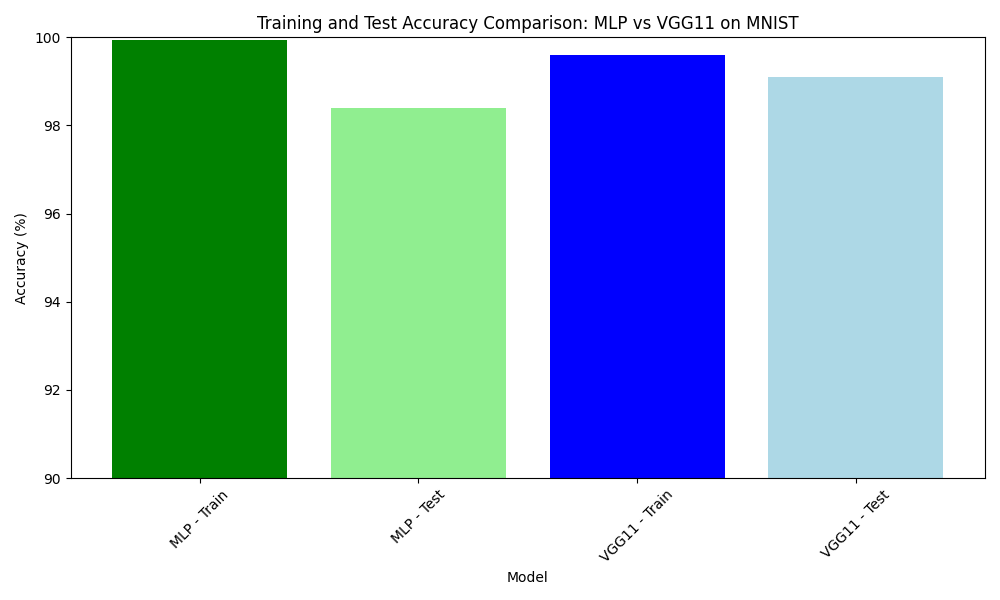
\includegraphics[width=0.8\textwidth]{mlp_vs_vgg11_train_test_accuracy_comparison.png}
    \caption{Final Training and Test Accuracy Comparison: MLP vs VGG11 on MNIST}
    \label{fig:mlp_vgg11_comparison}
\end{figure}

On the other hand, the VGG11 model also achieved very high training and test accuracies. But, unlike the MLP model, the difference between the train and test accuracies is very small. This tells me that VGG11 generalizes better to the test data, showing less overfitting compared to the MLP.

In the line plot (Figure \ref{fig:vgg11_mlp_accuracy}), which shows the accuracy over the training epochs, it is clear that both models perform well. The MLP model, however, had a bit more fluctuation in its accuracy, while VGG11's accuracy remained more stable throughout the training. This stability means that VGG11 is better at consistently improving over epochs without sudden drops, which is a good sign of effective training.

\begin{figure}[H]
    \centering
    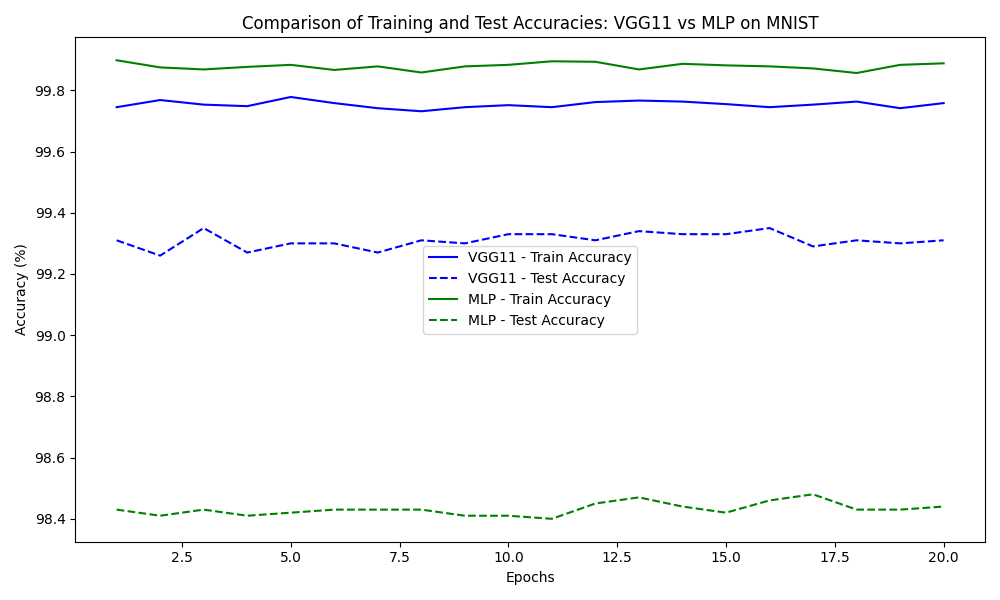
\includegraphics[width=0.8\textwidth]{vgg11_vs_mlp_accuracy.png}
    \caption{Comparison of Training and Test Accuracies: VGG11 vs MLP on MNIST}
    \label{fig:vgg11_mlp_accuracy}
\end{figure}

\subsection{Overall Comparison}
It seems that VGG11 slightly outperformed MLP in terms of both accuracy and stability. This result makes sense because VGG11 is a more complex convolutional model, which is generally better suited for image classification tasks like MNIST. The MLP model still did a good job, but it showed some signs of overfitting and was a bit less stable compared to VGG11.

\section{Exercise 2, Question 4: Introduction}
In this part of Exercise 2, I modified the architecture of the Multi-Layer Perceptron (MLP) and trained it on the MNIST dataset for 20 epochs. The modifications involved adding additional fully connected layers, as well as introducing Batch Normalization and extra ReLU activations to the network. This modification aimed to improve the model's performance by enhancing its learning capacity and reducing overfitting.

\section{Exercise 2, Question 4: Results and Analysis}
The results of the modified MLP training process are shown in Figures \ref{fig:modified_mlp_accuracy} and \ref{fig:modified_mlp_loss}. Based on these plots, I made several observations:

\begin{figure}[h]
    \centering
    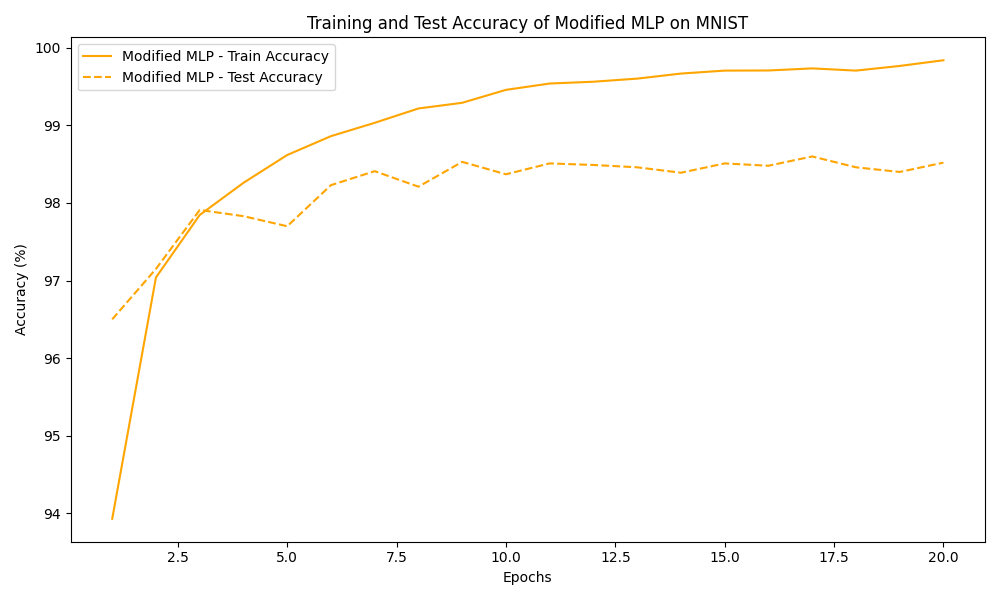
\includegraphics[width=0.8\textwidth]{modified_mlp_accuracy.png}
    \caption{Training and Test Accuracy of Modified MLP on MNIST}
    \label{fig:modified_mlp_accuracy}
\end{figure}

\begin{figure}[h]
    \centering
    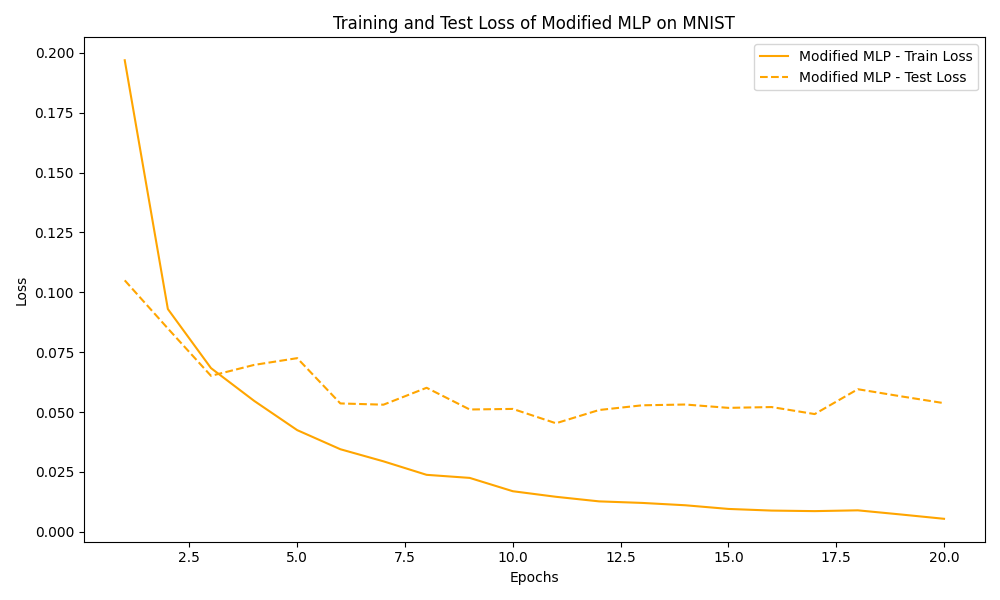
\includegraphics[width=0.8\textwidth]{modified_mlp_loss.png}
    \caption{Training and Test Loss of Modified MLP on MNIST}
    \label{fig:modified_mlp_loss}
\end{figure}

\subsection{Accuracy and Loss of Modified MLP}
The modified MLP showed consistent improvement in training accuracy over the epochs, reaching a value close to 100\%. The test accuracy, on the other hand, remained slightly lower but showed stable performance. The training and test loss also decreased over time, indicating that the model was successfully minimizing its error on both the training and validation data.

\subsection{Comparison with Original MLP}
Figure \ref{fig:mlp_comparison} shows the comparison between the original MLP and the modified MLP. The modified MLP achieved higher training accuracy compared to the original model, indicating that it was better at learning the training data. Additionally, the modified model also achieved improved test accuracy, showing a notable difference compared to the original MLP. This indicates that the changes made to the architecture helped the model generalize better on unseen data.

\begin{figure}[H]
    \centering
    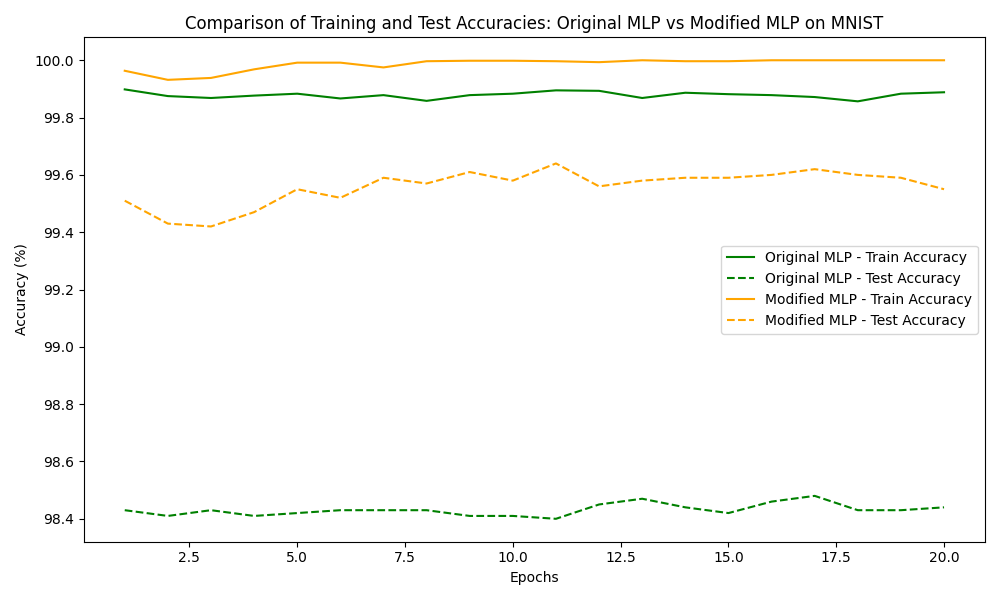
\includegraphics[width=0.8\textwidth]{mlp_vs_modified_mlp_accuracy.png}
    \caption{Comparison of Training and Test Accuracies: Original MLP vs Modified MLP on MNIST}
    \label{fig:mlp_comparison}
\end{figure}

\section{Exercise 2, Question 4: Conclusion}
Overall, the modifications to the MLP model resulted in improved training accuracy and higher test accuracy. The addition of more layers and Batch Normalization helped the model better learn from the training data while also improving generalization capabilities. The gains in test accuracy suggest that the architectural changes positively impacted the model's performance on unseen data, making it a more robust solution compared to the original MLP.




\section{References}
\begin{itemize}
    \item PyTorch documentation: \url{https://pytorch.org/}
    \item Torchvision datasets: \url{https://pytorch.org/vision/stable/datasets.html#mnist}
\end{itemize}




\vspace{+0.5cm}

%\par \textbf{Acknowledgement}\\

%I would like to acknowledge that I used ChatGPT to help \underline{refine my grammar and sentence structure} in this document. However, the \underline{solutions and ideas presented here are entirely my own}. 


\end{document}
              